\section[Proof of Proposition 5.17]{Proof of Proposition~\ref{prop-enclosing-ellipse}}
\label{app-enclosing-ellipse}

We prove Proposition~\ref{prop-enclosing-ellipse}, whose statement we 
reproduce here.

\begin{un-proposition}
  Let $A$ be a bounded convex subset of $\R^2$ with non-empty
  interior. Then there exists an ellipse $E$ such that $A\seq E$, and
  such that 
  \begin{equation}\label{eqn-area-EA}
    \area(E) \leq \frac{4\pi}{3\sqrt 3}\area(A). 
  \end{equation}
\end{un-proposition}

\begin{proof}
  We may assume without loss of generality that $A$ is compact, for it
  it is not, we can replace $A$ by its closure, which has the same
  area as $A$ because $A$ is convex. Let $\Disk$ be the closed unit
  disk, and consider the collection $\Aff(A,\Disk)$ of all affine
  transformations $f:\R^2\to\R^2$ satisfying $f(A)\seq\Disk$. Then
  $\Aff(A,\Disk)$, with the natural topology, is a compact
  set. Therefore, there exists some $f\in\Aff(A,\Disk)$ maximizing the
  area of $f(A)$.  We claim that $f$ is invertible. Indeed, since $A$
  is bounded, there exists some $\lambda>0$ such that $\lambda
  A\seq\Disk$. Since $\lambda A$ has non-zero area, and multiplication
  by $\lambda$ is an affine map, it follows that $f(A)$ has non-zero
  area as well, and so $f$ is invertible. Let $E=f^{-1}(\Disk)$. We
  claim that $E$ is the desired ellipse.
  \[ \m{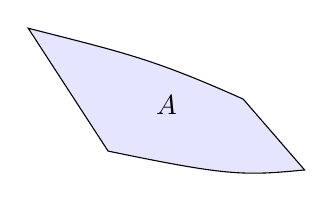
\begin{tikzpicture}[scale=1.5,cm={1.3,-0.5,0,0.5,(0,0)}]
    \draw[fill=blue!10] (1,0) -- (0.6,0.8) .. controls (0,0.9) and (-0.2,0.8)
    .. (-0.8,0.6) 
    -- (-0.28,-0.96) .. controls (0.5,-0.6) and (0.6,-0.5) .. (1,0) --
    cycle;
    \draw (0.1,0.2) node {$A$};
    \def\dot#1{\draw (#1) node {$\bullet$};}
  \end{tikzpicture}}
  \quad\xmapsto{\makebox[8mm][c]{$f$}}\quad
  \m{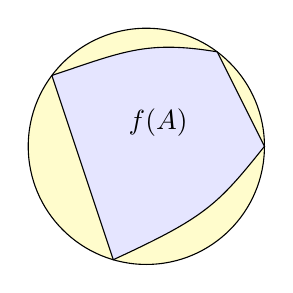
\begin{tikzpicture}[scale=1.5]
    \draw[fill=yellow!20] (0,0) circle (1);
    \draw[fill=blue!10] (1,0) -- (0.6,0.8) .. controls (0,0.9) and (-0.2,0.8)
    .. (-0.8,0.6) 
    -- (-0.28,-0.96) .. controls (0.5,-0.6) and (0.6,-0.5) .. (1,0) --
    cycle;
    \draw (0.1,0.2) node {$f(A)$};
    \draw (-0.6,-0.8) node[left=2mm] {$\Disk$};
    \def\dot#1{\draw (#1) node {$\bullet$};}
  \end{tikzpicture}}
  \quad\xmapsto{\makebox[8mm][c]{$f^{-1}$}}\quad
  \m{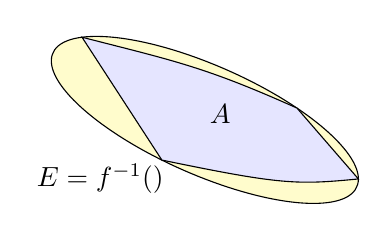
\begin{tikzpicture}[scale=1.5,cm={1.3,-0.5,0,0.5,(0,0)}]
    \draw[fill=yellow!20] (0,0) circle (1);
    \draw[fill=blue!10] (1,0) -- (0.6,0.8) .. controls (0,0.9) and (-0.2,0.8)
    .. (-0.8,0.6) 
    -- (-0.28,-0.96) .. controls (0.5,-0.6) and (0.6,-0.5) .. (1,0) --
    cycle;
    \draw (0.1,0.2) node {$A$};
    \draw (0,-1) node[left=4mm] {$E=f^{-1}(\Disk)$};
    \def\dot#1{\draw (#1) node {$\bullet$};}
  \end{tikzpicture}}
  \]
  We have $A\seq E$ by construction. We must show
  {\eqref{eqn-area-EA}}. Because affine transformations preserve ratios
  of areas, we may equivalently show
  \[ \area(\Disk) \leq \frac{4\pi}{3\sqrt 3}\area(f(A)).
  \]
  Let $\del\Disk$ be the boundary of $\Disk$, and consider points $p$
  where $f(A)$ ``touches'' the boundary, i.e., points $p\in f(A)\cap
  \del\Disk$. We claim that any arc segment of $\del\Disk$ of length
  $2\pi/3$ radians ($120$ degrees) contains at least one such
  point. To prove this, assume, for the sake of contradiction, that
  there is such an arc segment $Q$ not containing any point of
  $f(A)$. By rotational symmetry, we may without loss of generality
  assume that $Q$ is the arc from $-\pi/3$ to $\pi/3$ radians on the
  unit circle. Let $z_1$ and $z_2$ be the endpoints of $Q$, as shown here:
  \[
  \m{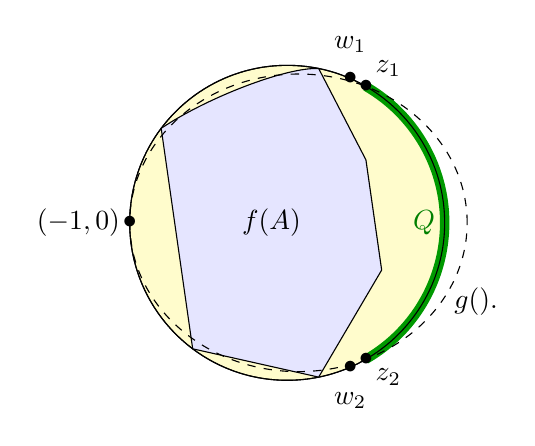
\begin{tikzpicture}[scale=2]
    \draw[fill=yellow!20] (0,0) circle (1);
    \draw[line width=1.2mm, color=green!60!black] (0.5,-0.8660254037) arc (-60:60:1);
    \draw (0,0) circle (1);
    \draw[fill=blue!10] 
    (0.2,-.9797958971) -- (0.6,-0.3) -- (0.5,0.4) -- (0.2,.9797958971) .. controls (0,0.99) and (-0.5,0.8)
    .. (-0.8,0.6) 
    -- (-0.6,-0.8) -- (0.2,-.9797958971) --
    cycle;
    \draw[dashed, cm={1.0714285714,0,0,.9449111825,(.0714285714,0)}] (0,0) circle (1);
    \draw (1,-0.5) node [right] {$g(\Disk)$.};
    \draw (-0.1,0) node {$f(A)$};
    \draw (1,0) node[left, color=green!50!black] {$Q$};
    \draw (-0.6,-0.8) node[left=2mm] {$\Disk$};
    \def\dot#1{\draw (#1) node {$\bullet$};}
    \dot{0.4,.9165151389};  \draw (0.4,.9165151389) node[above=2mm] {$w_1$};
    \dot{0.4,-.9165151389}; \draw (0.4,-.9165151389) node[below=2mm] {$w_2$};
    \dot{0.5,.8660254037};  \draw (0.5,.8660254037) node[above right] {$z_1$};
    \dot{0.5,-.8660254037}; \draw (0.5,-.8660254037) node[below right] {$z_2$};
    \dot{-1,0}; \draw (-1,0) node[left] {$(-1,0)$};
  \end{tikzpicture}}
  \]
  Since both $Q$ and $f(A)$ are compact, there exists some $d>0$ such
  that the distance between any point of $A$ and any point of $Q$ is
  at least $d$. Let $w_1$ and $w_2$ be the two points on the unit
  circle whose distance from $Q$ is $d/2$. Now consider the affine
  transformation $g$ that fixes $(-1,0)$ and maps $w_1$ to $z_1$ and
  $w_2$ to $z_2$. Then $g(\Disk)$ is an ellipse whose boundary passes
  through the points $(-1,0)$, $z_1$, and $z_2$, shown as a dashed
  line in the above illustration. It is therefore bisected by
  $Q$. Since the map $g$ moves no point of the unit disk by more than
  distance $d$, the set $g(f(A))$ does not intersect $Q$. It follows
  that $g(f(A))$ is contained in $\Disk$. On the other hand, a
  calculation shows that the area of $g(f(A))$ is slightly greater
  than that of $f(A)$, contradicting the assumption that the area of
  $f(A)$ was maximal.

  We have proved that every arc segment of length $2\pi/3$ radians on
  the boundary of $\Disk$ contains a point of $f(A)$. It follows that there
  is some finite cyclic sequence of points $p_1,\ldots,p_n\in f(A)\cap
  \del\Disk$ such that consecutive points are no more than $2\pi/3$
  radians apart. By connecting each $p_i$ to the center, we partition
  each of the sets $f(A)$ and $\Disk$ into $n$ pieces $B_1,\ldots,B_n$ and
  $C_1,\ldots,C_n$, respectively.
  \[
  \m{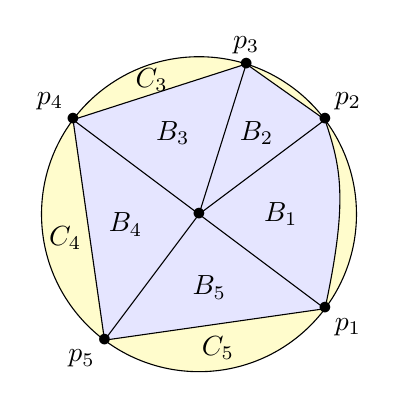
\begin{tikzpicture}[scale=2]
    \draw[fill=yellow!20] (0,0) circle (1);
    \draw[fill=blue!10] (0.8,-0.6) .. controls (0.95,0.1) and
    (0.9,0.3) .. (0.8,0.6) -- (0.3,.9539392014) -- (-0.8,0.6) 
    -- (-0.6,-0.8) -- (0.8,-0.6) --
    cycle;
    \draw (0.52,0) node {$B_1$};
    \draw (.366,0.518) node {$B_2$};
    \draw (-0.166,.518) node {$B_3$};
    \draw (-.466,-.066) node {$B_4$};
    \draw (.066,-.466) node {$B_5$};
    \draw (-.3,.85) node {$C_3$};
    \draw (-.85,-0.15) node {$C_4$};
    \draw (.12,-.85) node {$C_5$};
    \def\dot#1{\draw (#1) node {$\bullet$};}
    \dot {0,0};
    \dot {0.8,-0.6};    
    \draw(0.8,-0.6) node[below right] {$p_1$} -- (0,0);
    \dot {0.8,0.6};     
    \draw(0.8,0.6) node[above right] {$p_2$} -- (0,0);
    \dot {0.3,.9539392014};   
    \draw(0.3,.9539392014) node[above] {$p_3$} -- (0,0);
    \dot {-0.8,0.6};    
    \draw(-0.8,0.6) node[above left] {$p_4$} -- (0,0);
    \dot {-0.6,-0.8};   
    \draw(-0.6,-0.8) node[below left] {$p_5$} -- (0,0);
  \end{tikzpicture}}
  \]
  The fact that the inner angles are less than $2\pi/3$ immediately
  implies that $\area(C_i)\leq \frac{4\pi}{3\sqrt 3}\area(B_i)$ for
  all $i$; hence also $ \area(\Disk) \leq \frac{4\pi}{3\sqrt
    3}\area(f(A))$. This finishes the proof of the proposition.
\end{proof}


